\documentclass{llncs}
\usepackage{graphicx}
\usepackage{placeins}
%
\begin{document}
\pagestyle{headings} 
\mainmatter
%
\title{Hybrid Approach Based on Combination of Backpropagation and Evolutionary Algorithms for Artificial Neural Networks Training by Using Mobile Devices in Distributed Computing Environment}
%
\author{Iliyan Zankinski, Maria Barova, Petar Tomov}
%
\authorrunning{Iliyan Zankinski} 
%
\tocauthor{Iliyan Zankinski, Maria Barova, Petar Tomov}
%
\institute{Institute of Information and Communication Technologies\\
Bulgarian Academy of Sciences\\
acad. G. Bonchev Str, Block 2, 1113 Sofia, Bulgaria\\
\email{iliyan@hsi.iccs.bas.bg}}
%
%Iliyan Zankinski iliyan@hsi.iccs.bas.bg
%Maria Barova m.barova@iit.bas.bg
%Petar Tomov p.tomov@iit.bas.bg 
%
\maketitle
%
\begin{abstract}
When Evolutionary Algorithms (EAs) are used for Artificial Neural Networks (ANNs) training, the most valuable advantage is the potential for this training to be done in parallel or even using distributed computing. With the capabilities of modern mobile devices, for example their use for distributed computations, they can be used much more extensively for scientific calculations. It is well known that distributed computing systems are limited by their communication bandwidth, because of network latency. In such environment some EAs are pretty suitable for distributed implementation. This is because of their high level of parallelism and relatively less intensive network communication needs. Subset of distributed computing is volunteer computing where users donate some of the computing power provided by devices under their control. This research proposes Android Live Wallpaper volunteer computing implementation of a system used for financial time series prediction. The forecasting module is organized as ANN, which is trained by hybrid combination of Backpropagation and EAs. 
\keywords{Artificial Neural Networks, Evolutionary Algorithms, Distributed Computing}
\end{abstract}
%
\section{Introduction}
%
ANNs are very common in the field of machine learning. In its nature ANN training is an optimization problem. When the searching space is too big EAs for global optimization as Genetic Algorithms (GAs) can be very suitable. In the last two decades there are alot of attempts to combine EAs based optimization with the ANNs training. This combination shows to be much more promising when it is implemented as distributed computing system [2,5,6]. With the rising popularity of the mobile devices a lot of new possibilities for distributed computing can be investigated. Successful desktop distributed computing projects [3,4] can be efficiently implemented on mobile devices. This idea can be applied on EA based ANN training into a mobile distributed computing environment [1]. In this paper genetic algorithm in combination with backpropagation artificial neural network training is described. The training is done on a mobile devices as active Android wallpaper application. In addition, the traditional ANN's sigmoid function is replaced by fading sinusoidal function. The successful application of this hybrid approach is documented by series of experiments.

This paper is organized as follows. Section 1 gives an overview of the problem  with a special emphasis on ANNs/GAs and their strengths/weaknesses when applied for the problem's solution. Section 2 introduces a distributed computing environment based on mobile devices. Experiments and results are presented in Section 3. The final Section 4 concludes and some further work suggestions are provided. 
%
\subsection{Time Series Forecasting Problem}
%
%
\subsection{Artificial Neural Networks}
%
%
\subsection{Genetic Algorithms}
%
%
\section{Mobile Devices Distributed Computing}
%
\begin{figure}
	\centering
	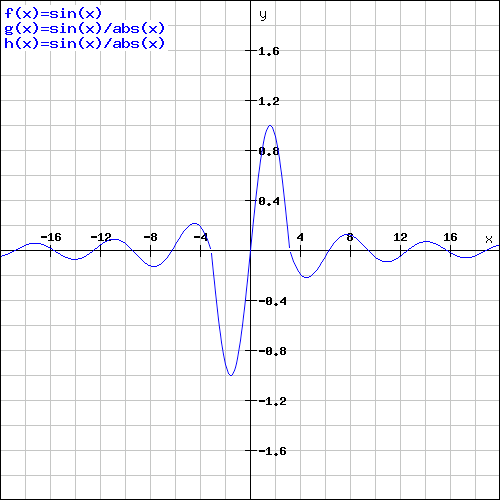
\includegraphics[width=7.88cm,height=7.88cm]{fig01.png}
	\caption{Fading sine function.}
	\label{fig:Graph}
\end{figure}
%
\begin{figure}
	\centering
	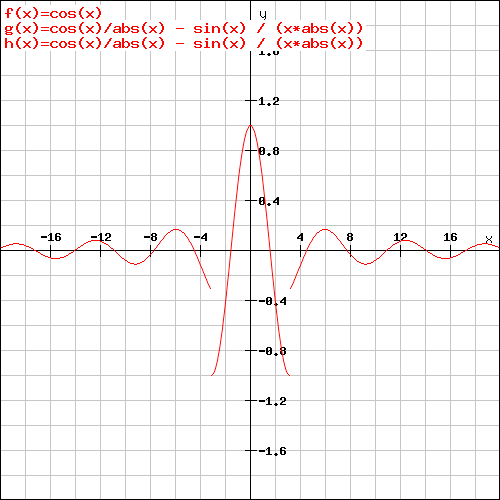
\includegraphics[width=7.88cm,height=7.88cm]{fig02.png}
	\caption{Fading sine derivative.}
	\label{fig:Graph}
\end{figure}
\FloatBarrier
%
\section{Experiments and Results}
%
%
\section{Conclusions}
%
%
\section*{Acknowledgements}
%
This work was supported by private funding of Velbazhd Software LLC.
%
% ---- Bibliography ----
%
\begin{thebibliography}{}
%
\bibitem {bal:zan:1}
Balabanov, T., Zankinski, I., Barova, M.:
VitoshaTrade Distributed Computing Android Wallpaper.
https://github.com/TodorBalabanov/VitDisComp Sofia, Bulgaria  (2017)
%
\bibitem {bal:zan:1}
Balabanov, T., Zankinski, I., Barova, M.:
Strategy for Individuals Distribution by Incident Nodes Participation in Star Topology of Distributed Evolutionary Algorithms.
Cybernetics and Information Technologies, Sofia, Bulgaria, vol. 16, no. 1, 80--88  (2016)
%
\bibitem {bal:1}
Balabanov, T.:
Distributed evolutional model for music composition by human-computer interaction.
Proceedings of International Scientific Conference UniTech15, University publishing house V. Aprilov, Gabrovo, Bulgaria, vol. 2, 389--392 (2015)
%
\bibitem {bal:2}
Balabanov, T.:
Avoiding Local Optimums in Distributed Population based Heuristic Algorithms (in Bulgarian).
Proceedings of XXIII International Symposium Management of energy, industrial and environmental systems, John Atanasoff Union of Automation and Informatics, Sofia, Bulgaria, 83--86 (2015)
%
\bibitem {bal:dob}
Balabanov, T., Zankinski, I., Dobrinkova, D.:
Time Series Prediction by Artificial Neural Networks and Differential Evolution in Distributed Environment.
International Conference on Large-Scale Scientific Computing, Sozopol, Bulgaria, Lecture Notes in Computer Science, vol. 7116, no. 1, 198--205  (2011)
%
\bibitem {bal:3}
Balabanov, T.:
Heuristic Forecasting Approaches in Distributed Environment (in Bulgarian).
Proceedings of Anniversary Scientific Conference 40 Years Department of Industrial Automation, UCTM, Sofia, Bulgaria, 163--166 (2011)
%
\end{thebibliography}
\end{document}
